\documentclass[10pt,a4paper]{article}

\usepackage[margin=1.65cm,top=1.4cm,bottom=1.5cm]{geometry}
\usepackage{amsmath,amssymb}
\usepackage{graphicx}
\usepackage{booktabs}
\usepackage{xcolor}
\usepackage[hidelinks]{hyperref}
\usepackage{caption}
\usepackage{titlesec}

\captionsetup{font=small,labelfont=bf,skip=2pt}
\titleformat{\section}{\normalfont\bfseries}{\thesection}{0.6em}{}
\titlespacing*{\section}{0pt}{5pt}{1pt}
\setlength{\parskip}{2.5pt plus 1pt}
\setlength{\parindent}{0pt}
\setlength{\abovedisplayskip}{3pt}\setlength{\belowdisplayskip}{3pt}
\setlength{\abovedisplayshortskip}{1pt}\setlength{\belowdisplayshortskip}{2pt}
\setlength{\textfloatsep}{6pt plus 2pt}

\newcommand{\code}[1]{\texttt{#1}}
\newcommand{\Gf}{G_{\mathrm f}}
\newcommand{\Gb}{G_{\mathrm b}}
\newcommand{\topk}{\operatorname{TopK}}
\newcommand{\PH}[1]{\textcolor{red}{[#1]}}

\begin{document}

{\centering
{\large\bfseries Why a 24-layer stream-bottleneck model does not train, and how to make it train}\\[1pt]
{\small TinyStories; \(d=1024\), \(N=4096\), \(K=512\), MD optimizer, lr \(3\!\cdot\!10^{-4}\), 20k steps.
Full record, all runs and negative results: \code{docs/stream-bottleneck-depth-journal.tex}.}\par}

\section{Observation}

Each block ends in a stream bottleneck: with the block's residual contribution
\(\Delta_\ell(x)=a_\ell+\mathrm{MLP}_\ell\bigl(\mathrm{RMSNorm}(x+a_\ell)\bigr)\), \(a_\ell=\mathrm{Attn}_\ell\bigl(\mathrm{RMSNorm}(x)\bigr)\),
\begin{equation*}
  x_{\ell+1}=\mathcal N\bigl(B(x_\ell+\Delta_\ell(x_\ell))\bigr),\qquad
  B(h)=g_DW_DP_{S(h)}W_Eh,\quad S(h)=\topk_K|W_Eh|,
\end{equation*}
\(\mathcal N\) an optional RMSNorm (post-norm); nothing routes around \(B\).  With 8 layers the model trains.
With 24 layers and a post-norm, validation CE stays at 5.95--5.97 for 10k steps: the unigram entropy of the
corpus is 5.9665 nats, so the output does not depend on the input.  Without the post-norm the 24-layer runs end
at CE \(=\ln 50257\) with zero gradient.  A backward-preserving decoder scale, MD gain spreads, orthogonal
initialization and shared projections all left this unchanged.

\section{First mechanism: the selection gain}

\(B\) is positively homogeneous and piecewise linear: \(B(h)=J(h)\,h\) with \(J=g_DW_DP_SW_E\), the autograd
Jacobian.  At initialization \(z=W_Eh\) is Gaussian and the encoder rows and decoder columns have unit norm and
are nearly orthogonal, so \(\|h\|^2\approx d\,\overline{z^2}\) (\(\overline{z^2}\): the mean over all \(N\)).
Forward, each kept neuron carries its own value \(z_i\); backward, the same \(K\) neurons carry
\(u_i=w_{D,i}^\top g\), and a gradient unrelated to the selection has \(\mathbb E\,u_i^2=\|g\|^2/d\):
\begin{equation}
  \Gf=\frac{\|B(h)\|^2}{\|h\|^2}\approx\frac{g_D^2\sum_{i\in S}z_i^2}{d\,\overline{z^2}}=g_D^2\,\frac Kd\,s^2,
  \qquad
  \Gb=\frac{\|J^\top g\|^2}{\|g\|^2}\approx\frac{g_D^2\sum_{i\in S}u_i^2}{\|g\|^2}=g_D^2\,\frac Kd,
  \label{eq:gains}
\end{equation}
\begin{equation}
  \frac{\Gf}{\Gb}=s^2(\rho)=\frac{\operatorname{mean}_{i\in S}z_i^2}{\operatorname{mean}_i z_i^2}
  =\mathbb E\bigl[Z^2\,\big|\,|Z|>t_\rho\bigr]=1+\frac{2t_\rho\,\varphi(t_\rho)}{\rho},
  \qquad \rho=\tfrac KN,\ \ t_\rho=\Phi^{-1}\bigl(1-\tfrac\rho2\bigr).
  \label{eq:s2}
\end{equation}
Both passes go through the same \(K\) neurons, so \(K/d\) cancels; the forward carries the \emph{largest}
coefficients, a selection-blind gradient typical ones (a random \(K\)-subset would give 1).  \(s^2=4.02\) at
\(K/N=1/8\) and 8.90 at \(K=32\); the measured ratio matches \eqref{eq:s2} to 0.5--3\,\% from \(K=32\) to 2048
(Fig.~\ref{fig:init}a).  A scalar \(c\) --- \(g_D\), the MD gains, or a post-norm (\(c=\sqrt d/\|B(h)\|\) per token) ---
multiplies both gains by \(c^2\), and an orthogonal init or shared weights leaves \(z\) Gaussian: the architecture
fixes only the ratio, \(\prod_\ell\Gf^{(\ell)}/\Gb^{(\ell)}=s^{2L}\) for every choice of scale.  The ratio is what
matters because the output depends only on the direction of \(x_L\) (final RMSNorm): a change \(\delta\) of the
stream at block \(\ell\) (new information, or an update of that block) reaches the output with relative size
\begin{equation}
  \frac{\|\delta_L\|/\|x_L\|}{\|\delta_\ell\|/\|x_\ell\|}=\prod_{m=\ell}^{L-1}\sqrt{\frac{\Gb^{(m)}}{\Gf^{(m)}}}=s^{-(L-\ell)} .
  \label{eq:depth}
\end{equation}
The scale only decides where \(s^{2L}\) appears.  Fixing \(\Gb=1\) (backward-preserving \(g_D\)) puts it in the
forward: \(\|x_L\|\propto s^L\) (\(1.6\cdot10^7\) at \(L=24\)), and training overflows \(x^2\) in float32 inside the
RMSNorms (CE \(=\ln V\)).  Fixing the forward (post-norm) puts it in the backward:
\(\|\partial\mathcal L/\partial x_\ell\|\propto s^{-(L-\ell)}\), \(\times2.1\) per block, a factor \(2.4\cdot10^{7}\)
between the last and the first block at initialization (Fig.~\ref{fig:init}b; 247 at 8 layers) and
\(3\cdot10^{12}\) at step 2000.

\section{Second mechanism: a renormalized carry collapses the tokens}

Removing the selection gain is not enough: every post-norm variant stays on the plateau, including a value
shift with \(\Gf=\Gb\) exactly (flat initial gradient), a near-critical surrogate backward (RBLapSum, \(T=1\)),
and \(K=N\) (no selection).  With the value shift every block moves at first, yet by step 2000 the streams of
all positions coincide from block 16 up and the gradient again decays \(\times2.3\) per block.  For the stream \(x_{b,t}\) of position \(t\) of sequence \(b\) entering a block and that block's
output \(\Delta_{b,t}\), with \(\bar v_b=\frac1{T'}\sum_{t\ge16}v_{b,t}\) the mean over the positions of a sequence,
\begin{equation*}
  f=\frac{\operatorname{mean}_b\|\bar x_b\|^2}{\operatorname{mean}_{b,t}\|x_{b,t}\|^2},\qquad
  r=\frac{\operatorname{mean}_{b,t}\|\Delta_{b,t}\|^2}{\operatorname{mean}_{b,t}\|x_{b,t}\|^2},\qquad
  r_c=\frac{\operatorname{mean}_b\|\bar\Delta_b\|^2}{\operatorname{mean}_{b,t}\|x_{b,t}\|^2}.
\end{equation*}
Exactly, \(1-f=\operatorname{mean}_{b,t}\|x_{b,t}-\bar x_b\|^2/\operatorname{mean}_{b,t}\|x_{b,t}\|^2\) is the energy share of
the token-specific deviations (\(f=1\) iff every position holds the same vector), and \(f\) is the norm-weighted
mean cosine over all pairs of positions,
\(f=\sum_{t,t'}\|x_t\|\|x_{t'}\|\cos(x_t,x_{t'})/(T'\sum_t\|x_t\|^2)\), i.e.\ \(f=\tfrac1{T'}+(1-\tfrac1{T'})\,\overline{\cos}\) when all
positions have the same norm, as after a post-norm.  \(r\) and \(r_c\) are the energies of a block's output and of
its token-independent part, relative to the carry.  The bottleneck multiplies a small \(f\) by the slope of its
correlation map, \(\kappa=\mathbb E[Z^2\mathbf 1(|Z|>t_\rho)]=\rho\,s^2(\rho)\) (0.50 at \(K/N=1/8\), 1 for
\(K=N\)).  A post-norm leaves \(f\) unchanged but resets the carry to unit RMS, so \(r\approx1.9\) at every depth
and \(f\) relaxes geometrically to a fixed point,
\begin{equation}
  f_{\ell+1}=\kappa\,\frac{f_\ell+r_c}{1+r}\ \ \Longrightarrow\ \
  f^\ast=\frac{\kappa\,r_c}{1+r-\kappa}.
  \label{eq:fstar}
\end{equation}
At initialization \eqref{eq:fstar} with the theoretical \(\kappa\) gives 0.010, 0.18, 0.84, 0.985 for
\(K=32\), 512, 2048, \(N\); measured 0.013, 0.20, 0.88, 0.99 (Fig.~\ref{fig:init}c).  With \(K=N\) the stream
is token-independent from the start; the same carry without a norm stays at 0.56, because there the carry
accumulates energy and \(r\) falls with depth (0.17 to 0.05).  With \(K=512\) the selection's decorrelation
holds \(f\) at 0.2 until training makes the top blocks emit the unigram: in the failed run at step 2000 their
outputs carry \(r=56\)--\(1.9\cdot10^4\) times the energy of the unit carry, all of it token-independent
(\(r_c/r\to1\), \(\kappa\to1\)), and in those blocks every position holds the same vector (cosine 1.000 for
essentially every pair; the untrained lower blocks keep their initial 0.2, and runs without a norm stay \(\le0.2\) in
every block, Fig.~\ref{fig:train}c), and
the bottleneck gain of those blocks (\(\Gf\) up to 2680) further divides the gradient below them.  The
first 13 blocks never moved (\(\|W-W_0\|/\|W_0\|<5\cdot10^{-4}\), falling \(\sim2\times\) per block; Adam's
\(\epsilon=10^{-8}\) against gradients of \(10^{-20}\)--\(10^{-16}\)).

\begin{figure}[t]
\centering
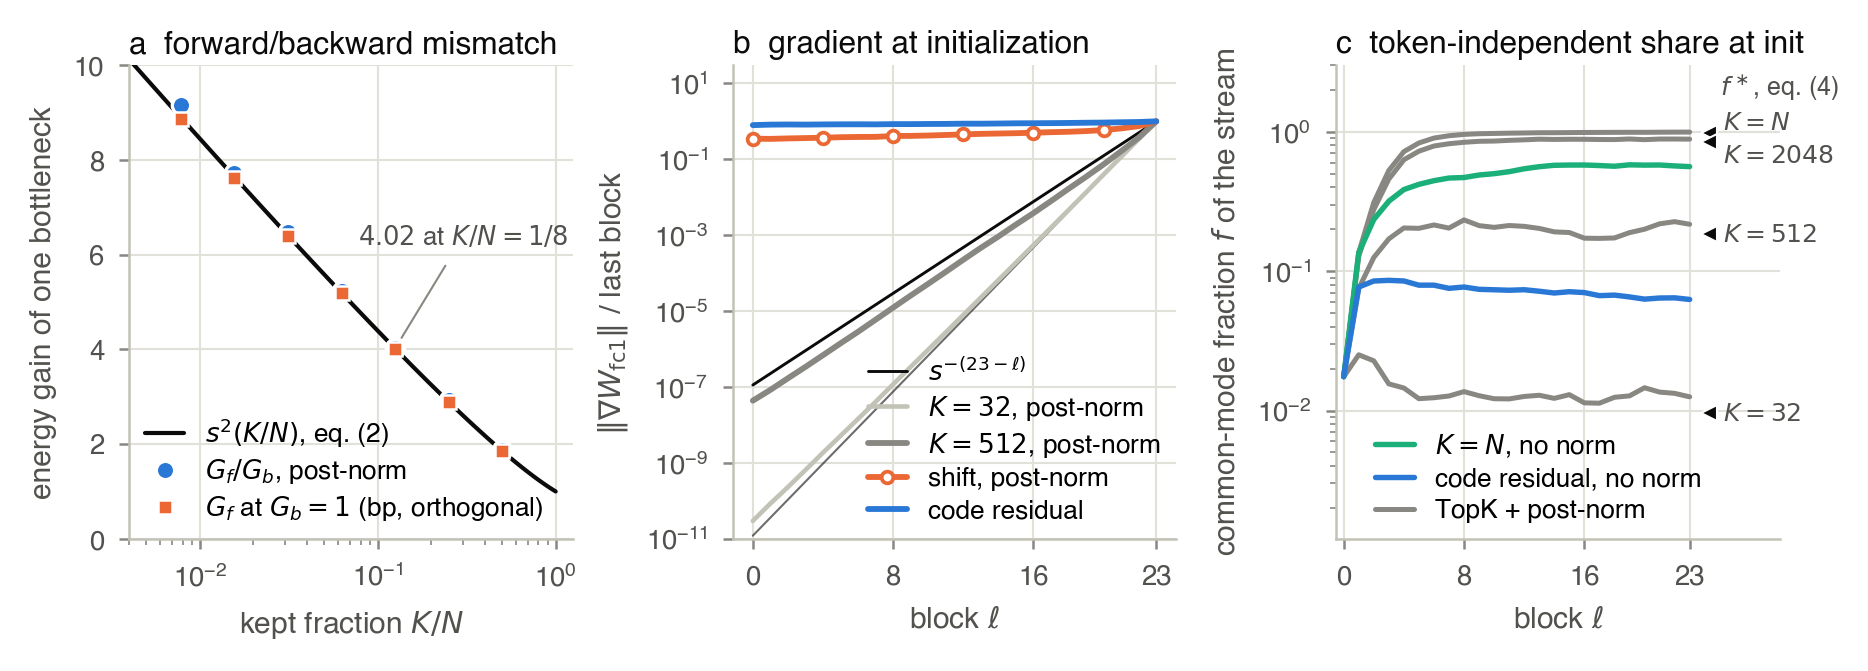
\includegraphics[width=\textwidth]{figures/depth/fig_init.png}
\caption{Initialization, 24 layers.  \textbf{a} Energy gain of one bottleneck against \eqref{eq:s2}.
\textbf{b} Gradient reaching block \(\ell\).  \textbf{c} Common-mode fraction of the stream; gray: post-norm
at four \(K\), with the fixed points \eqref{eq:fstar} (triangles).}
\label{fig:init}
\end{figure}

\section{Fix: remove the selection gain, then drop the post-norm}

The second mechanism asks for a carry that is not renormalized: a stream that accumulates energy, like a
pre-norm residual stream, turns a token-independent block output into a logit bias (\(r_\ell\) falls with depth)
instead of compounding it.  Dropping the post-norm, which was there to contain the forward half of
\eqref{eq:depth}, in turn requires removing the selection gain.  Two ways to do that
(\code{ActivationBottleneckConfig}), both keeping every stream between blocks an exactly (\(\le\))\,\(K\)-sparse
code; the second is the one we recommend.

\textbf{Value shift} (\code{value\_shift=energy}): keep the support and shrink the kept magnitudes,
\(y_i=\operatorname{sign}(z_i)\max(|z_i|-\delta,0)\), with \(\delta\) solved per token from
\(\operatorname{mean}_Sy^2=\operatorname{mean}_{\mathrm{all}}z^2\).  The Jacobian on the support is unchanged
and \(\Gf\) drops to \(\Gb\) (both \(1.00\pm0.01\) in every block at initialization).  It removes the selection
gain of \emph{Gaussian} codes only: training makes the kept magnitudes heavy-tailed, the shift must grow
(\(\delta/\sigma\): 1.04 to 1.95) and zeroes an increasing share of the support (56\,\% by step 7k), with
gradient spikes; a fixed \(\delta=\lambda^\ast\sigma\) falls out of balance and stalls.  It confirms the
mechanism but is not a robust fix.

\textbf{Code residual} (\code{code\_residual=true}): remove the reselection itself.  This was the natural idea from
the start: a deep stack trains when every block is the identity plus a small update, and a stream bottleneck
breaks exactly that --- each block re-encodes the stream and reselects from fresh Gaussian coefficients, which is
where the selection gain comes from.  Designed against the first mechanism, it also removes the second, because
nothing renormalizes the carried code.  Carry the code, with one shared dictionary,
\(c_0=\topk(W_Ex_{\mathrm{emb}})\), \(x_\ell=g_DW_Dc_\ell\), and only the block's contribution is encoded:
\begin{equation*}
  \text{original (no norm): } c_{\ell+1}=\topk\bigl(g_DW_E^{(\ell)}W_D^{(\ell-1)}c_\ell+W_E^{(\ell)}\Delta_\ell(x_\ell)\bigr),\qquad
  \text{code residual: } c_{\ell+1}=\topk\bigl(c_\ell+W_E\Delta_\ell(x_\ell)\bigr).
\end{equation*}
Plain \(\topk\), no shift and no post-norm.
\(\topk\) is the Euclidean projection onto \(K\)-sparse vectors, so a silent block is the identity and
\(\partial c_{\ell+1}/\partial c_\ell=P_{S_{\ell+1}}(I+\dots)\): a pre-norm residual network in code space, which
needs no norm on the carry.
Re-encoding the decoded stream is not idempotent (\(g_DW_E^{(\ell)}W_D^{(\ell-1)}\neq I\)), so the value shift meets only the first
two requirements: its carry alone (branches off) keeps the mean squared singular value at 1 but, as a product of
24 random rank-\(K\) maps, transmits the input along an effective 14 of 1024 directions; the code residual's carry
is the identity.

\section{Results}

\begin{figure}[t]
\centering
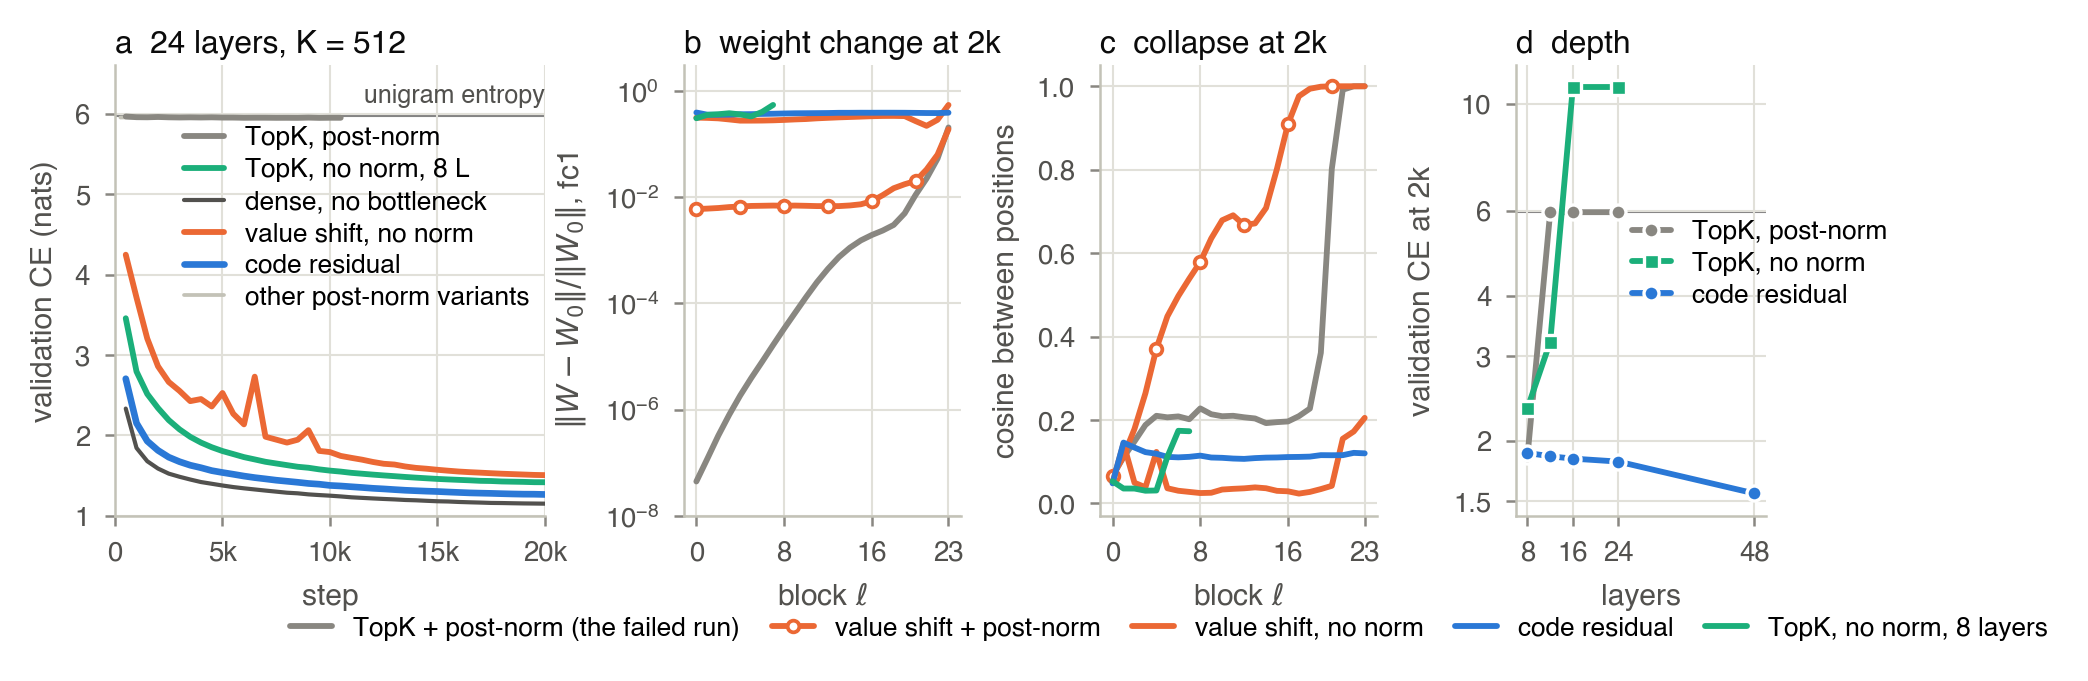
\includegraphics[width=\textwidth]{figures/depth/fig_training.png}
\caption{Training.  \textbf{a} Validation CE; light gray: all other post-norm variants (value shift energy/fixed,
shared projections, RBLapSum, \(K=32\), \(K=N\)).  \textbf{b,c} Checkpoints at step 2000: relative weight change
per block and cosine between positions.  \textbf{d} Validation CE at step 2000 against depth.}
\label{fig:train}
\end{figure}

Same data, schedule, seed and hyperparameters as the failed run (MD, lr \(3\cdot10^{-4}\), backward-preserving
\(g_D\)); only the architecture differs.

\begin{center}\small
\begin{tabular}{lccccc}
\toprule
validation CE (nats) & step 2k & step 20k & parameters & s/step \\
\midrule
24 L, TopK + post-norm (the failed run)          & 5.959 & 5.949 at 10.5k & 555M & 1.10 \\
24 L, code residual                              & 1.814 & 1.266 \ (seed 2: 1.267) & 362M & 1.03 \\
24 L, code residual, \(K=32\)                    & 2.107 & 1.517 & 362M & 1.01 \\
24 L, code residual, per-block projections       & 1.797 & 1.263 & 563M & 1.06 \\
24 L, value shift, no norm                       & 2.859 & 1.506 & 555M & 1.13 \\
24 L dense (no bottleneck)                       & 1.588 & 1.152 & 354M & 0.70 \\
8 L, TopK + post-norm                            & 1.862 & 1.348 & 219M & 0.45 \\
8 L, TopK, no norm (earlier reference)           & 2.340 & 1.418 & 219M & 0.45 \\
8 L, code residual                               & 1.890 & 1.361 & 161M & 0.49 \\
\bottomrule
\end{tabular}
\end{center}

With the code residual the 24-layer model trains to 1.266, below every 8-layer bottleneck model (best 1.348),
0.11 nats behind a dense 24-layer model, with 35\,\% fewer parameters than the failed model and the same step
time; the \(K=32\) configuration, previously stuck at 5.947, reaches 1.517.  It improves monotonically with depth
(Fig.~\ref{fig:train}d; val CE at 2k 1.890, 1.860, 1.839, 1.814, 1.558 at 8, 12, 16, 24, 48 layers), whereas TopK with
a post-norm trains at 8 layers and sits on the plateau from 12 on, and without a norm slows at 12 and overflows
from 16.  At step 2000 every post-norm run has collapsed positions and a vanishing gradient, every run without
one has neither (Fig.~\ref{fig:train}b,c).  The value shift trains at \(K=512\) but drifts, and reaches only 4.53 and
4.81 at 2k for \(K=32\) and 128.  An encoder/decoder pair per block instead of one shared pair reaches 1.263
at 20k against 1.266: 0.003 for 55\,\% more parameters (the two seeds of the shared model differ by 0.001).

\textbf{Conclusion.}  The 24-layer model did not fail because \(K=512\) removes information (\(K=N\) fails the same
way with a post-norm), but because the stream bottleneck replaces the residual identity path: its selection gain
\(s^2(K/N)\), which no scale can remove, forced a post-norm, and the renormalized carry collapses the tokens.  Carrying
the \(K\)-sparse code between blocks restores the identity path, keeps every stream exactly \(K\)-sparse, and makes
depth pay off.  Single seeds except the 24-layer code residual; TinyStories, 20k steps.

\end{document}
